\documentclass[a4paper,12pt]{article}
\usepackage{ctex}
\usepackage{geometry}
\geometry{a4paper, left=2.5cm, right=2.5cm, top=2.5cm, bottom=2.5cm}
\usepackage{amsmath, amssymb}
\usepackage{enumerate}
\usepackage{graphicx}
\usepackage{float}

\title{Reinforcing Spatial Reasoning in Vision-Language Models with Interwoven Thinking and Visual Drawing}
\author{Yang}

\begin{document}
\maketitle

\section{Introduction}
Ablation study(消融实验):拆掉模型或算法的某些部分,探究其对性能的影响

当下的LVLM推理模型推理来源仍然是文本,仅依赖模型将图片视频转化为文本再进行推理。但是困难在于这样的转化是必然有损失的,无论是将视觉信息转化为文本还是文本对于动态演变的事物的描述不能做到面面俱到。创新之处在于让模型在每一部推理过程可以使用训练过的drawing技能编辑视觉信息,同时补充空间细节和关系

最新的相关研究选择集成视觉处理工具,但一方面视觉工具是黑盒,另一方面依赖于人类先验处理的数据,过于简单化

创新模型功能:绘制用于定位的边界框和用于分析的辅助线

模型训练框架:
\begin{itemize}
    \item 用合成数据去训练模型基本的绘制功能
    \item 设计了reflective rejection sampling mechanism,用于让模型根据中间结果纠正行为(提升模型自我纠正能力)
    \item 强化学习(提高整合能力且保证单次推理的优秀)
\end{itemize}

\section{Related Work}
Visual Spatial Reasoning除了需要视觉感知能力之外,还需要关系推理(理解物体间的空间位置关系)和视角变换(保持和操纵空间变化)

\section{Methodology}
\subsection{Reasoning}
输入问题$Q$,以及图像输入$\{I_n\}$,要求给出输出$A$。当给予模型$M$输入的时候,模型会生成reasoning path $R = \{(r_t, e_t, o_t)\}$,分别表示自然语言推理、绘画操作和执行绘画操作之后的观察结果,直到推理出一个结论性结果

模型具备的两个绘画操作:bounding box annotation和auxiliary lines drawing。对于每个操作都包含三个参数:
\begin{itemize}
    \item $k$:目标图像索引($\{I_n\}$中的哪一个),无论是来自原图像还是来自上一推理路径给出的$o_t$
    \item $p$:单个或多个用于操作的坐标
    \item $l$:描述注释内容的语义标签
\end{itemize}

在执行每一步推理时会产生$r_t$和$e_t$,后者的产生基于整个交互历史,且$e_t$中包含$m_t$个操作。可以将$e_t$理解为一个向量,向量的分量之间存在时序关系,每个分量代表一个操作,需要操作的索引,操作的坐标和操作的批注,操作之后会产生一个影响,也就是$o_t$,也可以理解为一个向量,具有时序关系

\subsection{Training}
训练关注选择题和计数问题(是具有代表性还是说研究存在局限性,需要考察OOD情况)

reward function:$S = 1(S_{correct} > \beta) * (S_{correct}(A, \hat{A}) + S_{format})$,其中$\beta$表示一个threshold(阈值),保证准确性至少要大于阈值才可以算上标准型分数(防止模型进入reward hack获取更高的format分数来降低accuracy)。$\hat{A}$代表期望答案,对于选择题:$S = 1(A = \hat{A})$,对于计数问题:$S = \frac{1}{|C|}\sum_{\theta \in C}1(\frac{|A - \hat{A}|}{A} < 1-\theta)$,其中$C$是MRA这种奖励计算方法的水平集合,大致为$C = \{0.5, 0.55, \dots, 0.95\}$,检查$A$和$\hat{A}$之间的relative error是否在阈值内,可以做到测量模型在不同严格度下的精确度。对于$S_{format}$,如果输出的操作是可执行的,那么就给$1$,否则为$0$

cold training:定义$L_n = E_{I, Q, A, R, D_{cold}}(-\frac{1}{N}\sum_{t=1}^{T}logp(r_t, e_t|R_{<t}, I, Q))$,其中$N = \sum_{t=1}^{T}(|r_t| + |e_t|)$,表示执行操作的总token数,目的要让$L_n$最小化

dataset:首先收集图片和视频的问题对,然后用模型进行推理路径生成,然后根据定义的score公式筛选高质量的空间推理数据

reflective rejection sampling:需要定义什么是反思行为,在本论文中定义为不同时间步骤下同一标签再次出现但是行为不同,即$\exists(t_1, t_2, u, v): (l_{t_1}^{u} = l_{t_2}^{v}) and (e_{t_1}^u != e_{t_2}^{v})$,可以理解为$t_1$时刻第$u$个行为的标签与$t_2$时刻第$v$个行为的标签一致,但是行为却不一致。经过cold training训练后的模型$M_{cold}$很少表现出这样的反思,这会影响到后面的RL过程,因此需要改进

improvement:定义\(L_{reflect} = E_{(I, Q, A) with D_{reflect}, R with M_{cold}(|I, Q)}(-\frac{1}{N}\sum_{t=1}^{T}log p(r_t, e_t | I, Q, R_{<t}))\phi\),其中$D_{reflect}$是一个给定的用于提升反思能力的数据集,然后用$M_{cold}$去进行微调,且$\phi$是一个二分筛选器,$\phi=1$当且仅当除了满足上面提出的准确性要求,格式要求之外还要求满足reflect任务

RL:采用训练策略的同时监视reasoning process,提前终止出现的无效和循环的推理过程,终止条件包括:
\begin{itemize}
    \item 模型没有输出任何执行操作且无法到达一个conclusive结果
    \item 累计图像的数量超过了预定义的阈值
    \item 重复执行了之前执行过的操作(存疑,也可以没有,毕竟执行的操作只有两类,画边框和画辅助线,但是否可以松弛化,比如辅助线依赖两个坐标,如果两次操作坐标的距离很小,换句话说两个辅助线之间几乎没有什么差距,那么是否也可以提前终止)
\end{itemize}
在RL训练的时候使用之前定义的reward function,使用GRPO策略进行训练,公式较为复杂:
\begin{figure}[H]
    \centering
    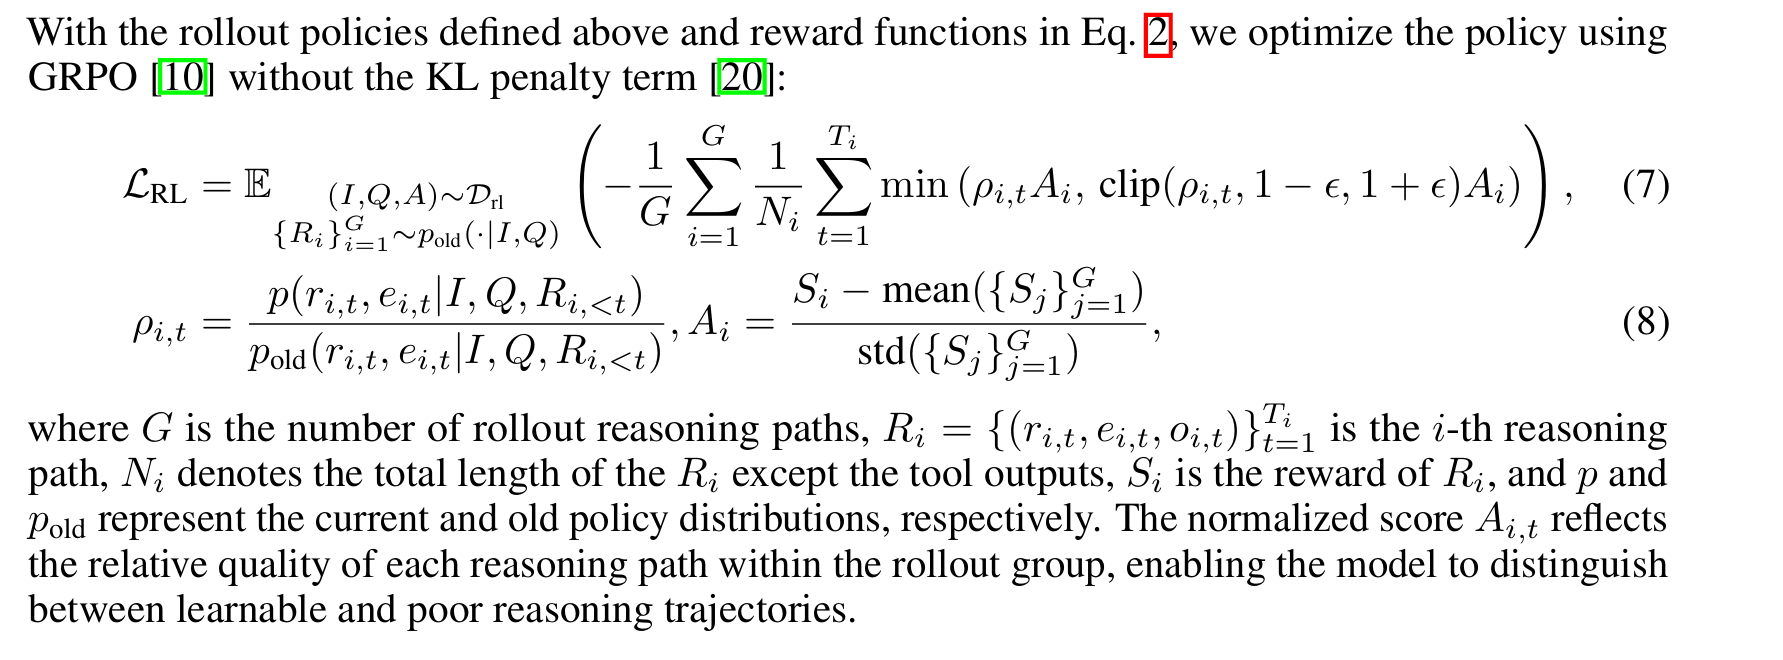
\includegraphics[width=\textwidth]{equation.png}
\end{figure}

\section{Expriment}
\subsection{setup}
从image、video和multi-view三个角度设置benchmark

\subsection{implementation}
使用Qwen(是否存在模型基础间的差异),训练的时候分辨率256*28*28,视频采样16帧,而测试的时候除了个别平台保持不变,其他保持16帧以及最大分辨率448*28*28,另外设置了最大处理图像数(因为在操作过程中,每一步操作都会生成一个副本而不是在原图上做出修改,但是反过来,是否需要保留原图,以及原图删除之后是否会影响反思回退逻辑还有待思考)

结果表示训练出的模型对于性能具有显著的提升,且Tool一列表示模型是否具备使用工具编辑图像的能力,而Reasoning表示模型是否使用推理功能

结论:
\begin{itemize}
    \item 闭源模型的推理能力要明显优于开源模型
    \item 本论文设计出的模型一方面可以将大任务进行可解释化拆解,并可以进一步捕捉追踪,而现有模型一方面依赖于感知工具,一方面不能做到反思和监督
\end{itemize}

Ablation study:研究反思逻辑展示、推理步骤数目、画边界框的数目和画辅助线的数目,可以理解为评价指标
结论:
\begin{itemize}
    \item Cold Training:是进行spatial reasoning的基础,没有这一步表现甚至比原来的基础模型还要差
    \item reflection sampling:显著提升了自我纠正能力,如果没有这一步骤,模型会快速的得出没有经过验证的画辅助线的操作
    \item RL:一方面帮助模型更有选择性地进行绘图操作,减少不必要的操作,且对于一些对数字精度更高的任务表现得更好
\end{itemize}

\subsection{Inference Scaling}
术语:pass@k(并行输出k个结果,取最好的那一个),当k足够大时反应模型能力的经验上限,而k=1时反应模型单次尝试的性能,而RL可以降低pass@k和pass@1之间的差距

Inference Scaling:指模型推理过程中的资源投入,本论文中可以理解为投入Cold Training,reflection sampling和RL,这些中间训练策略都是资源的投入,可以归为Inference Scaling(存疑)

结论:模型训练的前两个步骤对于两个指标都有提升,而RL除了提升之外还降低了两者之间的差距

\section{Summary}
本篇论文主要阐述了一种新的让多模态模型在面对视觉任务时具有更好的推理能力的训练策略。传统的方法是先将图像或视频信息转化为文本,再进行文本推理,但存在转化损失和难以应对动态变化场景的问题,而如果集成工具就存在黑盒难以监视的问题。本文提出的新的训练策略是引入绘图操作训练,让模型直接对视觉信息进行推理。引入的操作有画边界框定位和画辅助线分析。模型的训练主要包含三个环节:Cold Training(让模型学会最基本的绘图操作),Reflective Rejection Sampling(让模型提升其自我纠正能力,让反思步骤尽可能地出现),RL(使用定制的reward function进行训练,提升性能)。对于Cold Training环节,定义了一个公式,该公式的含义是基于给出的图像和问题以及前面的推导过程和操作过程,得出正确答案的概率的负对数和,当这个loss function最小化的时候说明模型选择正确操作的概率更高,因此模型具备了更好的spatial reasoning基础。而在Reflective环节,模型需要在最小化loss的基础上满足出现反思操作的要求。而在RL阶段进行训练,定义loss function和reward function,最大化reward score,最小化loss function
\end{document}